\documentclass[11pt]{article}
\usepackage{graphicx}
%opening
\title{Quanta Serialization Protocol}
\author{H.Ardaki}

\begin{document}

\maketitle


\section{Introduction}

In the following subsections i will try to justify use cases of \textbf{qsp} which stands for \underline{\textit{Quanta Serialization Protocol}}, answer some common questions and introduce a little insight about it


\subsection{What is qsp?}

qsp is a binary serialization protocol (or translation, depending on context)
its a set rules which will act as an isomorphism from set of all native objects to set of all byte-arrays\\
qsp is reversable as definition of isomorphism implies (Figure 1)\\
qsp can also be considered as a homomorphism for each 
equivalence classes of set of all native objects under equivalence relation of "instance of Type"\\\\
what is the difference between homomorphism and isomorphism and why its only homomorphic on a set of all instances of a certion type?\\
because qsp is type agnostic, it can potentially generate the same byte-array for two instances of different types (isomorphic does not promise its a one-to-one relation) but will never generate an equal byte-array for two unequal instance of a same type, and vice versa (figure 1.a)
we will heavily relay on above definition!
\pagebreak

\begin{figure}[h]
	\centering
	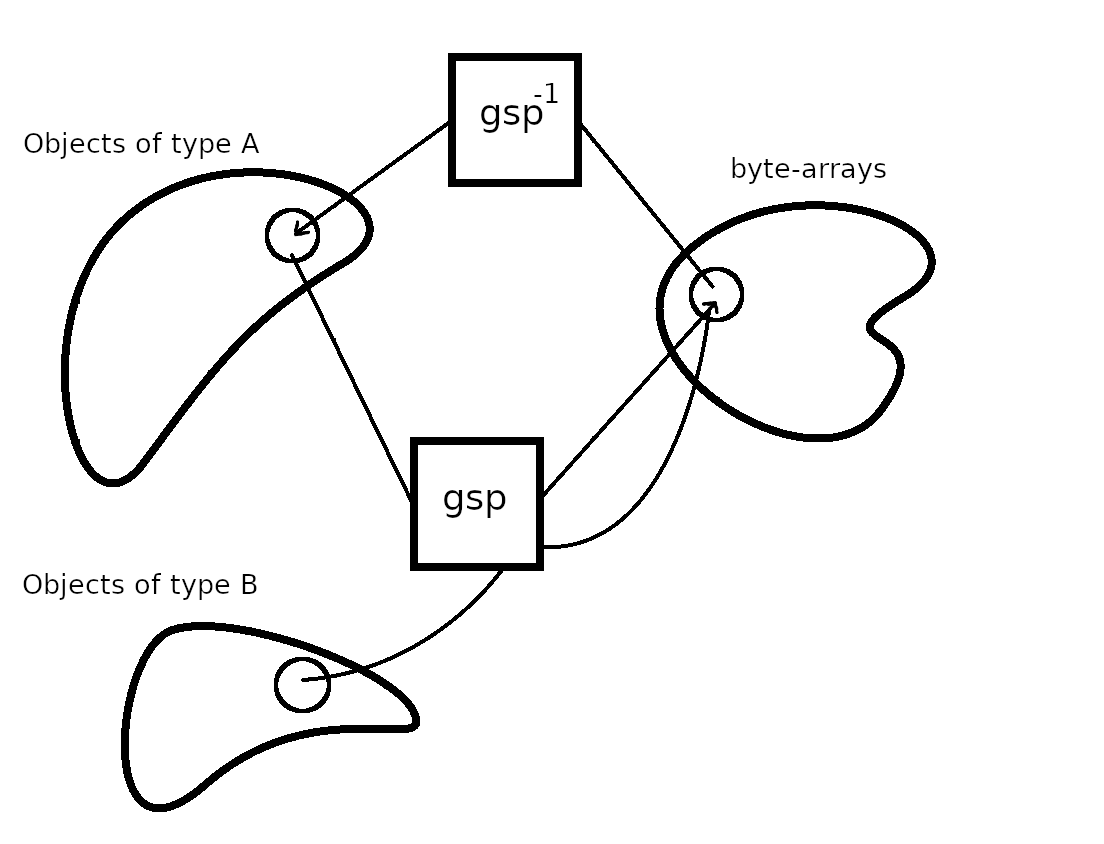
\includegraphics{gsp_iso.png}
	\caption{}
\end{figure}

\subsection{When and Where qsp is relevant?}
qsp will grab your object and freeze it as is and ignores any meta-data like type-flags or fields index or name, it will only use size indicators for dynamic fields (like strings or arrays) and everything else is fixed size for it and no padding or anything else will be around it\\\\
with above specifications qsp is not size efficient as other (similar) protocols might be, but it can perform faster conversions as the trade of.\\\\
computers are becoming more and more powerful and someone might says "it doesnt matter if i use couple of more thousands of CPU cycles to achieve the same result with an easier protocol" and thats true,but qsp can be used when you need that couple of thousands of CPU cycles for something else\\
some of qsp potential use cases:
\begin{itemize}
	\item HFT programming
	\item embedded systems
	\item IPC and memfiles
\end{itemize}



\end{document}
